\chapter{SecureWilly: Design and Implementation}
\begin{figure}[h!]
   \centering
   
\includegraphics[width=0.45\linewidth]{./figures/trt.png}
   \caption{Trademark of SecureWilly}
\end{figure}

\section{User Interface}

SecureWilly's user interface at the moment is rather simple and is represented by a terminal UI.

The user is given instructions at every step and is informed about the rules that must be followed in order to produce an AppArmor profile successfully.

Single service, as well as multi-service projects are supported. There are specific instructions about the forms of syntax of Dockerfile commands and Docker Compose options that are supported by SecureWilly, described in the corresponding sections. The user has the choice not to use Dockerfiles and Docker Compose file for his project, but is obligated to provide the docker commands that will be used for the project.

In order to use SecureWilly, user has to copy the directory Parser on host machine, under a directory where project's Dockerfiles and Docker Compose file exist. The script SecureWilly\_UI which is under the Parser directory has to be executed and the UI will direct user through the whole process.

\subsection{Input}
SecureWilly takes input adjusted on a particular application and uses it to run its static and dynamic parsers and eventually create an AppArmor profile adjusted on the needs of the application and the configuration of docker container(s).

First of all, SecureWilly asks the user to give the number of services that need a profile for the upcoming project. A service is defined by a docker image, either it is built by Dockerfile or is based on an existing image, with or without docker-compose file. Then the user is asked to write the names of each service. If Docker Compose file is used, the services should be identical to the ones used in yml file and given in the same order. If Docker Compose file has not been used, a service's name should be the name of the image used by docker run or docker create commands. Moreover, the names should be unique and not used for other purposes like named volumes, network etc.

Secondly, SecurilyWilly asks if any Dockerfiles are used for each service. The user is prompted to answer \say{N}, if there is no Dockerfile for a service, or give the path to Dockerfile if it exists.

Afterwards, the user is asked to do the same for Docker Compose file. If it exists, the path to it should be given, otherwise the answer should be \say{N}.

All of the requirements up to now, were related to static analysis. Hereupon, SecureWilly requires material related to dynamic analysis part.

SecureWilly will then ask the user whether a network is needed for the project. The answer should be either \say{N} for no, or the network's name for positive answer.

The last part of SecureWilly's requirements is a test plan of the project. The user is prompted to write the basic commands that will be used to run the container, including starting and stopping it and the commands in-between. A script is created, including these commands, and will be used as a test plan to train the application and produce system logs for dynamic analysis.

\subsection{Editing}
As soon as SecureWilly is done with user's input, starts the editing part.

The names of services are used in dynamic analysis so that the profiles produced have corresponding names to the services/images. They are also used to identify the part of yml file or the docker commands that refer to each service. 

The Dockerfiles are getting parsed the way they are in static analysis. If there is no Dockerfile for a service, an empty file is given to static parser.

Docker Compose file gets divided in mini docker compose files for each service and each one is given to static parser.

The network's name is used to create the network with docker command at the beginning of a run in dynamic analysis and is removed at the end of it.

Lastly, the test plan that the user is asked to provide, will be used in dynamic analysis to train the services and produce system logs. Moreover, if there is no Docker Compose file, the test plan will be used to detect the runtime flags used in docker commands, to create mini yml files for each service.

\subsection{Output}
SecureWilly produces one profile for each service. A directory, called parser\_output is created in the parent directory of Parser, and contains the services' profiles produced. It also contains the mini yml files for each service, as they me be helpful for the user, if willing to create a Docker Compose file. System logs produced from dynamic analysis are included also as well as all the versions of the profiles produced at each run of dynamic analysis.

The user should now copy the profiles in AppArmor directory (usually /etc/apparmor.d/) and load them in kernel. Then the option security\_opt should be added in Docker Compose file, or flag security-opt (--security-opt "apparmor:service\_profile") inside docker run/create commands.

\section{Static Analysis}
\subsection{Purpose}
The purpose of static analysis is to extract a set of rules from the initiative code of docker image in order to form a preliminary AppArmor profile.

Ideally, the initiative code of a docker image should provide most of the information about the task that the container intends to work on. Docker's concept differs from other virtualization types because it is supposed to run as a process. Therefore if we gather together all the actions we want to make inside the initiative code then the docker container would complete its task immediately and SecureWilly would be informed in a great extent of the container's desired actions.

Of course, there are more complex images, which require more complicated actions like running on interactive containers or sharing network between services etc and thus, not all images' tasks could be gathered together in the initiative code. In this case, we try to extract as many rules as we can in the static analysis phase, and let the profile be enriched in the dynamic analysis phase.
 
What makes static analysis invaluable, is that the rules extracted are not always seen in the system logs that are being examined in dynamic analysis. This derives from the fact that some of these rules are based on human logic assumptions, such as multiple use of USER instruction in Dockerfile. Furthermore, they speed up SecureWilly's performance since the preliminary profile includes rules that could possibly need more than one run of the testplan in order to be extracted in dynamic analysis. Therefore, the more rules SecureWilly achieves to extract in static analysis, the less runs will take place in dynamic analysis.

\subsection{Initiative code}
So where does that “initiative code” of docker images exist?
SecureWilly examines the following parts of docker images in order to create  a preliminary profile in the static analysis phase:

\begin{enumerate}
\item Dockerfile
\item Docker Compose (.yml file)
\item Runtime flags
\end{enumerate}

SecureWilly receives as input, all or whichever of these files are provided by the user (Runtime flags, is not actually a file, but the user is asked to provide some commands and a script is created out of them) and parses them in order to extract some AppArmor rules, as detailed in the following sections. 

\subsection{Dockerfile}
Our first approach was to examine Dockerfile. Dockerfile constitutes a \say{recipe} that tells Docker how to create the image for the container and so, it seemed like a smart idea to parse the documentation of Dockerfile searching for any points related to the isolation of a container. As soon as we detected such points, we tried to match them to AppArmor's documentation and extract some profile rules suitable for the respective docker image.

Dockerfile is a simple text file which includes the build instructions to build the image. The advantage of a Dockerfile over just storing the binary image (or a snapshot / template in other virtualisation systems) is that the automatic builds will ensure you have the latest version available. This is a good thing from a security perspective, as you want to ensure you're not installing any vulnerable software. \cite{whatsdockerfile}

Each Dockerfile builds the image of one service that will be run on a container. However, the AppArmor profiles that SecureWilly produces do not restrict any of the Dockerfile commands. The reason for this is that the image is getting built on the host, whereas the AppArmor profile we produce will be used to secure the container's process and thus the profile will only be enforced as soon as the container is up. This means that the Dockerfile can only give us some direction with its commands of what will the container do, but not exactly its actions.

Bearing in mind that our goal is maintaining host-container isolation, we pointed out some \say{commands} (Docker uses the term instructions instead of commands, as Dockerfile is an instruction file like we mentioned before) that could be used to extract the respective AppArmor rules.

These \say{commands} are given below:
\begin{itemize}
\item VOLUME directories
\item EXPOSE ports
\item USER \& RUN useradd
\item RUN chmod file
\end{itemize}

We will discuss each one of them below.

\subsubsection{VOLUME}

The VOLUME instruction creates a mount point with the specified name and marks it as holding externally mounted volumes from native host or other containers. The value in its string form is a plain string with multiple arguments, such as VOLUME /var/log or VOLUME /var/log /var/db. There is also a JSON array form ([\say{/var/log/}]) but SecureWilly is only dealing with string forms, at the time of writing.

The docker run command initializes the newly created volume with any data that exists at the specified location within the base image.

The most direct way for a container to interfere with host's filesystem is through mounting volumes. Mounting a volume can allow container to see and sometimes edit files on host. Undoubtedly, this constitutes mounting volumes an issue that security tools should handle in order to preserve isolation. What SecureWilly could use from that command, is a matching between host's directory and container's directory. 

Regardless of the great importance of VOLUME command, we came to the decision to exclude it from SecureWilly's Dockerfile searching field. The reason for this is that this command could not provide us the matching we could use to extract an AppArmor rule, but only the container's directory which on its own does not extract a useful rule. The VOLUME instruction does not support specifying a host-dir parameter, but only the container directory. The host directory is declared strictly at container run-time, as it is, by its nature, host-dependent. This is to preserve image portability, since a given host directory cannot be guaranteed to be available on all hosts. For this reason, a host directory cannot be mounted from within the Dockerfile.  The mountpoint must be specified when the container is created or run and thus, we would return to it in Docker-compose and Runtime flags phase.

\subsubsection{EXPOSE}
The EXPOSE instruction informs Docker that the container listens on the specified network ports at runtime. It can be specified whether the port listens on TCP or UDP. If protocol is not specified, Docker sets it to TCP by default.

Forwarding ports, as well as networking in general, is by definition highly associated with isolation since containers can reach out to host or other containers through it. Therefore, if ports are exposed, it means that the container should be able to use tcp or udp networking. Networking should be restricted only to this type of protocols and deny any other networking. This can be done with AppArmor using rule network tcp or network udp.

Although the EXPOSE instruction does not actually publish the port to the host machine, SecureWilly allows tcp/udp networking, since exposing ports essentially gives authorization to publish them to host at runtime. It functions as a type of documentation between the person who builds the image and the person who runs the container, about which ports are intended to be published. Moreover, the exposed ports will be accessible to linked services on the same network, so networking rules in AppArmor profile are needed.

To actually publish the port when running the container, the -p flag should be used on docker run to publish and map one or more ports, or the -P flag to publish all exposed ports and map them to high-order ports.

At the time of writing, AppArmor does not have rules to restrict specific port bindings. It is in its future plans though to provide new rules on networking - see Chapter \textit{Future Work} - and SecureWilly keeps a list of the exposed ports, hoping that restricting specific port bindings will be among them. 

Apart from the expecting rules of port binding, SecureWilly keeps the exposed ports in order to check if one of them belongs to ports with port number below 1024, the so-called well-known ports. In that case, the container needs capability CAP\_NET\_BIND\_SERVICE in order to bind/listen to such ports. In Linux, it is not possible for non-root users to bind low port numbers, unless they have capability CAP\_NET\_BIND\_SERVICE.

All in all, what SecureWilly's static parser does when encounters EXPOSE command, is detecting which protocol between tcp and udp is used and if the port has port number below 1024 and for each case extracts the following rules: \textbf{network tcp} or \textbf{network udp} and \textbf{capability net\_bind\_service}.

\begin{mdframed}[backgroundcolor=tipcolor]
\textbf{Tip}: The docker network command supports creating networks for communication among containers without the need to expose or publish specific ports, because the containers connected to the network can communicate with each other over any port. Therefore, it is recommended to use internal networks for communication among containers.

If communication with the host is needed then port forwarding is the best practice to use and certainly, avoid runtime flag --net=host (see Chapter \textit{Attacks and Vulnerabilities: Disabling Namespaces}).
\end{mdframed}

\subsubsection{USER \& RUN useradd}
The USER instruction sets the user name (or UID) and optionally the user group (or GID) to use when running the image and for any RUN, CMD and ENTRYPOINT instructions that follow it in the Dockerfile. At the time of writing, SecureWilly deals only with user names and UIDs.

The RUN instruction will execute any commands in a new layer on top of the current image and commit the results. The resulting committed image will be used for the next step in the Dockerfile. Thus, RUN useradd will add a new user to our image.

Restricting the set of users that can run the docker image, would be very beneficial for our goal to preserve isolation. Unfortunately, user namespaces are not yet supported by AppArmor and rules that refer to specific users do not yet exist.
  
However, SecureWilly barely touches this issue by allowing container's process to switch between users, if it is considered to be appropriate. Static parser uses an algorithm to count the total number of unique users that are either used by USER instruction or added to the docker image by RUN useradd. If switching users is considered to be appropriate then SecureWilly allows it, by adding the two capabilities that are necessary to make it happen, CAP\_SETUID and CAP\_SETGID.

So the rules that are added in that case are \textbf{capability setuid} and \textbf{capability setgid}.
\subsubsection{RUN chmod}

As mentioned above, the RUN instruction executes the command given to it in Dockerfile, and so, obviously RUN chmod will commit chmod's task, which is no other than changing the access permissions of a file system object.

Undeniably, an AppArmor profile that is capable to restrict container's access to filesystem, has a positive impact on maintaining isolation.

Taking this into consideration, when SecureWilly encounters such a command,  static parser breaks down the permission bits given and creates one file rule for the owner of the file and one for others - a similar rule for owning group is not yet supported by AppArmor.

The rules that are extracted by RUN chmod for the owner and others respectively are the following:
\begin{description}[style=nextline]
\item[owner \textless path/to/file\textgreater{} \textless owner's permissions (ix, w, wix, r, rix, rw, rwix)\textgreater]
File rule for owner's pwrmissions.
\item[\textless path/to/file\textgreater{} \textless others' permissions (ix, w, wix, r, rix, rw, rwix)\textgreater]
File rule for other's (world) permissions.
\end{description}

\subsubsection{Example}
An example of a Dockerfile, containing most of the commands we discussed previously, is presented below:

\begin{lstlisting}[style=Dockerfile, caption={Dockerfile example for static analysis}]
FROM ubuntu:latest
MAINTAINER Fani Dimou <fani.dimou92@gmail.com>

#Exposing port 80 tcp
EXPOSE 80/tcp

#Test 1
#Create file hello
#Permissions: By default r to everybody, w only to root
RUN echo "Hello everybody" > hello

#Create 2 users, userA with password A, userB with password B
RUN useradd userA && echo "userA:A" | chpasswd
RUN useradd userB && echo "userB:B" | chpasswd

#Create file greetings
RUN echo "userA says Hello" > greetings

#Test 2
#greetings: userA owner
#Permissions: rwx to userA, r to others
RUN chown userA:userA /greetings
RUN chmod 744 /greetings

ENTRYPOINT /bin/bash
\end{lstlisting}
\hfill\break
The AppArmor profile created by static analysis is the following:
\hfill\break
\begin{lstlisting}[style=Dockerfile, caption={AppArmor profile for example Dockerfile in static analysis}]
#include <tunables/global>

profile dockerfile_info_profile flags=(attach_disconnected,mediate_deleted) {

	capability setuid,  #Needed to switch between users
	capability setgid,  #Needed to switch between users
	network tcp, #Allowing networking with ports forwarding
	capability net_bind_service,  #This capability is needed to bind a socket to well-known ports
	owner /greetings rwix,
	/greetings r,
	file,  #Allows access to containers filesystem
	/var/lib/docker/* r, #Access to layers of filesystem
	deny ptrace (readby, tracedby), #Confront container breakout attacks
}
\end{lstlisting}

In the following listings we compare two containers running the same image, which was built from the Dockerfile above. The first container runs unconfined, which means it runs without using any AppArmor profile, and the second runs with the profile SecureWilly created enforced. Each user - root, userA - will try to read (cat) and write (touch) the files created in Dockefile (hello and greetings).

The container starts with root, who will be the first user to try accessing the files:

\noindent\begin{minipage}{.49\textwidth}
\begin{lstlisting}[caption=Unconfined,style=terminal]
root@2801ad69a688:/# cat hello
Hello everybody
root@2801ad69a688:/# touch hello
root@2801ad69a688:/# cat greetings 
userA says Hello
root@2801ad69a688:/# touch greetings
\end{lstlisting}
\end{minipage}\hfill
\begin{minipage}{.49\textwidth}
\begin{lstlisting}[caption=Profile enforced,style=terminal]
root@d2c77ad8dfcd:/# cat hello  
Hello everybody
root@d2c77ad8dfcd:/# touch hello 
root@d2c77ad8dfcd:/# cat greetings 
userA says Hello
root@d2c77ad8dfcd:/# touch greetings 
touch: cannot touch 'greetings': Permission denied
\end{lstlisting}
\end{minipage}

In the execution of the unconfined container, root has full access to all files. On the other hand, when the profile is enforced, the permissions, as given in Dockerfile, are respected, and not even root can override them - only the owner of greetings, who is userA, has write permissions, neither root nor anybody else. 

Afterwards, userA will try to login and commit the same actions:

\noindent\begin{minipage}{.49\textwidth}
\begin{lstlisting}[caption=Unconfined,style=terminal]
root@2801ad69a688:/# su userA
$ whoami
userA
$ cat hello
Hello everybody
$ touch hello
touch: cannot touch 'hello': Permission denied
$ cat greetings
userA says Hello
$ touch greetings
\end{lstlisting}
\end{minipage}\hfill
\begin{minipage}{.49\textwidth}
\begin{lstlisting}[caption=Profile enforced,style=terminal]
root@d2c77ad8dfcd:/# su userA
$ whoami
userA
$ cat hello
Hello everybody
$ touch hello
touch: cannot touch 'hello': Permission denied
$ cat greetings
userA says Hello
$ touch greetings
\end{lstlisting}
\end{minipage}

The login of userA is successful, due to the capabilities setuid and setgid, which are added by default by docker, and are permitted by SecureWilly's profile in the second container. As expected, userA has read permission to hello but not write and has both read and write permissions to greetings file.

Switching users as well as permissions work perfectly, therefore the rules we extracted from Dockerfile constitute the profile useful and efficient.

\subsection{Docker Compose}
It is a fact that most of the parameters we would like to obtain are not given at build phase but at runtime. Therefore, the material that Dockerfile offers to static analysis is limited, due to portability issues. Runtime parameters would constitute a key factor to create strict and fine-grained AppArmor profiles that reach our goal of containers obeying the Principle of least privilege. Docker offers a solution to this issue, with Docker Compose.
\hfill\break

\begin{figure}[h!]
  \centering
   
\includegraphics[width=0.5\linewidth]{./figures/dockercompose.png}
   \caption{Trademark of Docker Compose}
\end{figure}

Docker Compose is a tool for defining and running multi-container Docker applications, by using a YML/YAML file (Both yml and yaml work, but SecureWilly uses only yml at the moment). The reason why a yml file is an invaluable tool in our hands is that it provides a configuration for the container which includes a set of parameters that should be given at runtime at docker.

The Docker Compose file configures multiple containers, indicating how they should be built and connected, and where data should be stored. When the YML file is complete, a single command builds, runs, and configures all of the containers (docker-compose up).

After examining the documentation of docker compose, we detected several configuration options that could be used in order to extract AppArmor rules. All of the options we describe below, refer to version 3 of the Compose file format, which at the time of writing, is the newest version.
The list of the options that SecureWilly is parsing currently, is given below:

\begin{itemize}
\item Volumes
\item Expose
\item Ports
\item Capabilities add/drop
\item Ulimits
\item Devices
\end{itemize}

SecureWilly parses the yml file, like Dockerfile was parsed, and for each option on the list, creates the corresponding AppArmor rules, as described below. Examples for docker compose options are omitted, because most of the options are included in Nextcloud's example, which is presented in last chapter.

\subsubsection{Volumes}
Docker compose file's configuration option \say{volumes} is exactly what we were missing from Dockerfile's instruction VOLUME. It specifies mount host's paths or named volumes and gives us the desired binding between host's directory and container's directory.

SecureWilly supports only the short syntax of this option. In the short syntax, the path on the host can be specified by an absolute path mapping or a path relative to the Compose file. Relative paths should always begin with \say{.} or \say{..}. User-relative paths are not supported yet.

Docker Compose gives user the choice to specify only the container's path and let the Engine create a volume but at the moment, SecureWilly assumes that the user gives both paths. Moreover, user can specify named volumes and SecureWilly's static parser will replace the named volumes with the real host path, since it is known that volumes are situated under the path /var/lib/docker/volumes/. 

Lastly, the read only access mode is supported, and in this case SecureWilly allows only read permission to the volume specified.

Taking these points into consideration, we concluded that  SecureWilly should four rules per volume.

Firstly, a file rule should be added in order to define the permissions on the volume inside the container. If container's volume, has the read-only access mode enabled, then the permission read is added, otherwise both permissions read and write are added. So the first rule is: \\\textbf{\textless container's mountpoint\textgreater{} r} or \textbf{\textless container's mountpoint\textgreater{} rw}.

The rest of the rules, refer to the mount itself. Let it be known that docker forbids mounting volumes on running containers. Mounting volumes is only possible when starting a container. Docker indicates that containers are supposed to be ephemeral so, should the need for mounting a volume on a running container arises,  it is recommended to destroy the container and then recreate it to update the volume. Therefore, the existing mount on a container does not seem to be facing any real dangers, and since our AppArmor profile can only restrict actions that take place after the container is up, it should probably be worthless to add any mount rules.

However,  there has been a lot of talk about if docker should eventually allow mounting on running containers, as many users are making requests to include this feature somehow in future versions.

All things considered, we concluded that the profile owes to be specific about the existing mounted volumes, even if they cannot be affected by new mounts on running container at the moment. Thus, when the static parser encounters the option volumes in yml file, SecureWilly extracts three more rules. One specifying the existing mounting, and two that forbid editing the existing mountpoint on host, either by umounting or by remounting it.
\begin{description}[style=nextline]
\item[mount \textless source host path\textgreater{} -\textgreater{} \textless container's mountpoint\textgreater{}]
This rule allows the specified mounting and no other volumes are allowed to be mounted if there is no rule that allows it.

\item[deny umount \textless container's mountpoint\textgreater{}]
This rule means that this mountpoint cannot be unmounted.

\item[deny remount \textless container's mountpoint\textgreater{}]
This rule means that this mountpoint cannot be remounted.
\end{description}

When the read-only access mode is enabled on container's directory, static parser adds the ro option on the first of the three rules. The profile then is enriched by the following rules:
\begin{description}
\item[mount options=ro \textless source host path\textgreater{} -\textgreater{} \textless container's mountpoint\textgreater{}]
\item[deny umount \textless container's mountpoint\textgreater{}]
\item[deny remount \textless container's mountpoint\textgreater{}]
\end{description}

\subsubsection{Expose}

The expose option is the exact match of the EXPOSE instruction of Dockerfile. It exposes container's ports without publishing them to the host machine, but they will only be accessible to linked services. Only the internal port - container's port - can be specified.

Static parser extracts the exact same rules as in Dockerfile's EXPOSE:
\begin{description}[style=nextline]
\item[network tcp]
This rule is added if tcp is specified for a port or if none protocol is specified, as tcp protocol is used, by default. It allows only tcp networking
\item[network udp]
This rule is added if udp is specified for a port. It allows only udp networking
\item[capability net\_bind\_service]
This rule is added if container's port has port number below 1024. It allows granting capability CAP\_NET\_BIND\_SERVICE.
\end{description}

\subsubsection{Ports}

Ports option is used to publish ports to host. You can either use a short syntax, or give a more detailed configuration. SecureWilly supports only the short syntax, where either both ports are specified (HOST:CONTAINER) or just the container port and an ephemeral host port is chosen by Docker Engine.

If a port binding AppArmor rule existed, then the option ports would make a difference from expose option, but since there is no such rule at the moment, ports option extracts the same rules as expose.

\begin{description}[style=nextline]
\item[network tcp]
This rule is added if tcp is specified for the container's port or if none protocol is specified, as tcp protocol is used, by default. It allows only tcp networking
\item[network udp]
This rule is added if udp is specified for the container's port. It allows only udp networking
\item[capability net\_bind\_service]
This rule is added if container's port has port number below 1024. It allows granting capability CAP\_NET\_BIND\_SERVICE.
\end{description}

\subsubsection{Capabilities add/drop}
Linux processes can be of two types, privileged or unprivileged and so can the docker container's process. As a privileged process, the container can bypass all kernel permission checks, whereas as an unprivileged process, it is subject to full permission checking based on the its credentials (usually: effective UID, effective GID, and supplementary group list).\cite{containercaps} It goes without saying that setting limits to container's privileges is a great advantage for defending isolation.

Linux divides the privileges associated with superuser into distinct units, known as capabilities, which can be independently enabled and disabled. Docker supports adding and dropping capabilities at runtime, so that containers can run with a reduced capability set. By default Docker drops all capabilities except for the following list: CAP\_CHOWN, CAP\_DAC\_OVERRIDE, CAP\_FSETID, CAP\_FOWNER, CAP\_MKNOD, CAP\_NET\_RAW, CAP\_SETGID, CAP\_SETUID, CAP\_SETFCAP, CAP\_SETPCAP, CAP\_KILL, \\CAP\_SYS\_CHROOT, CAP\_NET\_BIND\_SERVICE, CAP\_AUDIT\_WRITE. Every container starts granting this set of capabilities, and it's up to user to drop any of them or add more.

AppArmor profiles can restrict a process's privileges by allowing or denying the capabilities specified. Even if a docker container grants already the default set of capabilities or adds any other at runtime, it cannot use them unless AppArmor profile allows it with a specific rule for each capability. Needless to say that SecureWilly will add only the necessary capabilities that container needs and drop the rest.

There are two options in docker compose file referring to capabilities: cap\_add, which adds capabilities and cap\_drop, which drops capabilities. Static parser detects these options and the capabilities that they specify and extracts an allowing or denying rule respectively:

\begin{description}
\item[capability \textless capability in cap\_add\textgreater{}] or
\item[deny capability \textless capability in cap\_drop\textgreater{}]
\end{description}

When rule capability is used without specific capability (or deny capability), it means that all capabilities that are supported by AppArmor are allowed (or denied). So if static parser encounters option cap\_add: ALL (or cap\_drop: ALL), it extracts rule \textbf{capability} (or \textbf{deny capability}).

\subsubsection{Ulimits}

Limiting processes is important for running a stable system. If host's resources are not appropriately distributed to the running processes, the system's stability might be in danger, as well as the system's security and particularly, isolation. A single user who starts too many processes can make the system unusable for everyone else. For instance, a fork bomb constitutes a denial of service attack in which a process continually replicates itself until available resources are depleted. Evidently, setting limitations to the resources of docker containers' processes is mandatory.

There are two mechanisms that control system's resources: cgroups and ulimits. Control groups (cgroups) is a linux kernel feature that limits or allocates the resources of the controlling hosts (cpu, memory, disk I/O, etc.) to the process groups. The ulimit is a tool for restricting the number of various resources a process can consume. While the main objective of these mechanisms is similar, there are some significant differences between them, such as their target group. In fact, we should say that cgroups are considered for allocating resources among user-defined groups of tasks, while ulimit only works on a process level. Although, cgroups is undoubtedly a very useful feature, restricting resources per container process approaches more the idea of the ulimit tool. Moreover, there are no rules for cgroups yet in AppArmor, so that automatically excludes cgroups.

The ulimit shell command is a wrapper around the setrlimit system call and the underlying data structure which contains the limit information is called rlimit. Ulimit controls the soft and hard limits over the resources available to the shell and to processes started by it. A hard limit is the real upper limit that the user can never exceed. The soft limit, on the other hand, is a “warning” limit. It tells the user and the system admin that you are close to reach the danger level, which is the hard limit. Regular users can increase their soft limits up to the current hard limit, but can’t exceed that. They can decrease their soft limits to zero. Regular users can also decrease their hard limits to zero, but they can’t increase them.

The option ulimits in docker compose file, overrides the default ulimits for a container. You can either specify a single limit as an integer or soft/hard limits as a mapping. At the time of writing, SecureWilly supports only the full syntax which includes soft and hard limits. 

AppArmor rlimit rules control the hard limit of an application and ensure that if the hard limit is lowered that the soft limit does not exceed the hard limit value. If a profile does not have an rlimit rule associated with a given rlimit then the rlimit is left alone and regular access, including changing the limit, is allowed. However if the profile sets an rlimit then the current limit is checked and if greater than the limit specified in the rule it will be changed to the specified limit.

SecureWilly's static parser detects the resource and its hard limit in the yml file and extracts the following rule:
\textbf{set rlimit \textless resource type\textgreater{} \textless = \textless hard limit\textgreater{}}

\subsubsection{Devices}
In Linux, various special files can be found under the directory /dev. These files are called device files. One of the most important things to remember about these device files is that they are most definitely not device drivers. They are more accurately described as portals to the device drivers. Data is passed from an application or the operating system to the device file which then passes it to the device driver which then sends it to the physical device. The reverse data path is also used, from the physical device through the device driver, the device file, and then to an application or another device. \cite{devices}

Although they usually behave unlike ordinary files, they still remane files, as everything in Linux is a file and thus, a mapping between them is treated like a usual a mount. Therefore, we extract the same file rules, like we did in volumes.

The device option in yml file, includes a list of device mappings.

The rules static parser extracts for each mapping are the following:
\begin{description}
\item[\textless container's device path\textgreater{} rw]
\item[mount \textless host's device path\textgreater{} -\textgreater{} \textless container's device path\textgreater{}]
\item[deny umount \textless container's device path\textgreater{}]
\item[deny remount \textless container's device path\textgreater{}]
\end{description}

\subsection{Runtime flags}
Docker Compose is a useful tool which was of great assistance for our static parser. However, it is mostly used for multi-service projects. Users who intend to run one single container, rarely use a Docker Compose file. The options that the yml file includes can all be given as runtime flags at docker run/create command. 

Although yml files worked perfectly in our static analysis, we could not overlook the frequency of this situation, and so SecureWilly asks the user whether a Docker Compose file is used. If the answer is negative, the user is asked to write down all the docker commands with which the container will run. Afterwards, SecureWilly detects all the runtime flags that match the options we used in the searching field for Docker Compose, and creates a mini yml file for each container, containing the values of the runtime flags in the correct syntax. This simple mini yml file is given to static parser, and is treated exactly the same way as a regular yml file and the same rules are extracted for the preliminary AppArmor profile.

The runtime flags that match the Docker Compose options are the following:
\begin{itemize}
\item volumes: -v \textless source host path\textgreater{}:\textless container's mountpoint\textgreater{}
\item expose: --expose \textless port\textgreater{}
\item ports: -p \textless host's port\textgreater{}:\textless container's port\textgreater{}
\item cap\_add: --cap-add \textless capability\textbar ALL\textgreater{}
\item cap\_drop: --cap-drop \textless capability\textbar ALL\textgreater{}
\item ulimits: --ulimit \textless resource type\textgreater{}=\textless soft\textgreater{}:\textless hard\textgreater{}
\item devices: --device \textless host's device path\textgreater{}:\textless container's device path\textgreater{}
\end{itemize}

The rules extracted are already described in the previous section \textit{Docker Compose}. 

\section{Dynamic Analysis}

\subsection{Purpose}
Creating an AppArmor profile by relying only on security, without considering what a service actually needs in order to work, would lead to a worthless profile. The profile SecureWilly produces should forbid any redundant and detrimental action, but above all, it should allow the service to complete its task successfully. In order to create a balanced profile between security and efficiency, SecureWilly runs the service multiple times and adds the appropriate rules that make the profile strict, specific but efficient as well.

In the dynamic analysis phase of SecureWilly, we focus on listening to services' needs, directly. This is achieved by examining the system logs produced when running the containers. We ensure that the profile produced will contain all the rules needed for the container in order to run successfully, by training the project multiple times with a test plan. Each run will produce some rules, which will be adapted to the existing profile. The new rules will give the green light to more actions and subsequently, to new system logs. SecureWilly will repeat the procedure, until there are no new rules extracted from the system logs.
%not stop adding new rules, until there are no new logs produced.

SecureWilly's dynamic analysis is especially invaluable to multi-service projects because it creates profiles that are aware of the association and cooperation of all services of the project. Static analysis extracts rules for the profile of each service separately. On the other hand, dynamic analysis runs the whole project multiple times. Like detailed above, after every run, new rules are added to each profile, and the project runs again with the updated profiles until none of the services produces new rules out of the system logs. Throughout our research, we came to the conclusion that logs are not produced all in once, but by adding some new rules to at least one of the services of a project, will permit actions coming not only by that particular service, but by any service of the project and that will lead to new system logs and thus new rules for all services. That's how the services of a multi-service project cooperate and SecureWilly's dynamic analysis respects that and creates profiles adapted to the cooperation of services.

\subsection{Dynamic Parser}
SecureWilly uses a parser in dynamic analysis which keeps the information given by the user about the services and the test plan, runs the project within a loop and monitors the system logs. At the end of this parser, a directory called parser\_output is created and the final profiles are included in it.

The dynamic parser follows the next steps:
\begin{enumerate}
\item Copy the preliminary profile of static analysis in AppArmor's directory
\item Load the profile in kernel and set the profile to complain mode with aa-complain
\item Execute test plan (start, stop, in-between operations)
\item Monitor the system logs
\item Adjust the profile
\item Repeat from the beginning until there are no new rules extracted from the logs
\item Load the profile in kernel and set the profile to enforce mode with aa-enforce
\item Repeat steps 3,4,5
\item If there are new rules extracted from the logs repeat from the beginning
\item Service's profile is produced
\end{enumerate}

SecureWilly uses a series of scripts to commit all of the actions above. Scripts are generic and as soon as user gives input to the User Interface, they are edited so that they become adjusted to the number and names of the services of each project and include project's test plan.

The steps of dynamic parser are clearly presented in the following flowchart:

\hfill\break\hfill\break\hfill\break\hfill\break\hfill\break\hfill\break\hfill\break\hfill\break\hfill\break\hfill\break\hfill\break\hfill\break\hfill\break\hfill\break

\begin{figure}[hp!]
  \centering
   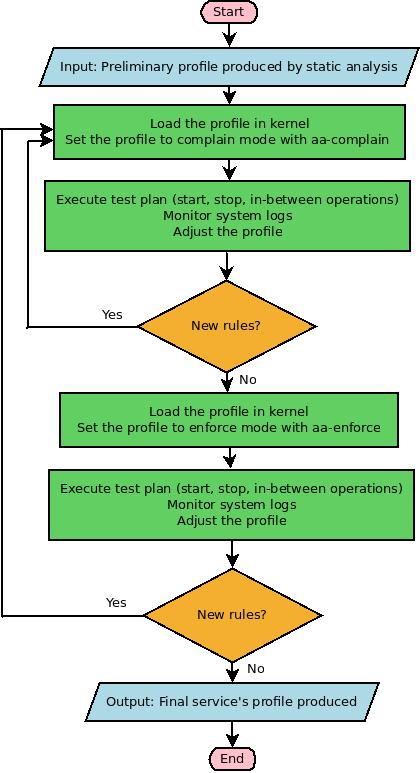
\includegraphics[width=0.8\linewidth]{./figures/DynamicAlgo.jpeg}
   \caption{Flowchart of dynamic parser}
\end{figure}

Let's take a closer look at the basic steps of dynamic parser.

\subsubsection{AppArmor profiles: load, complain, enforce}
The first operation of dynamic parser is to copy the preliminary profiles produced in static analysis to AppArmor's directory, which is usually located under /etc/apparmor.d/. An AppArmor profile should be loaded in kernel, in order to provide security. Thus, the profiles from static analysis are loaded into the kernel and replace any existing profiles with the same name, using the following command:

\begin{lstlisting}[style=dockercommands]
$ sudo apparmor_parser -r -W /etc/apparmor.d/<service_profile>
\end{lstlisting}

Afterwards, SecureWilly has to set the profile to one of AppArmor's modes. AppArmor profiles can be set to three different modes:

\begin{itemize}
\item In \textbf{audit mode}, security policy is enforced and all access (successes and failures) are logged to the system log. Command aa-audit is used to set an AppArmor profile to this mode.
\item In \textbf{complain mode}, security policy is not enforced but rather access violations are logged to the system log. Command aa-complain is used to set an AppArmor profile to this mode.
\item The \textbf{enforce mode}, is the default mode for a security policy. Command aa-enforce is used to set an AppArmor profile to this mode from being disabled by command aa-disable or from complain mode by command aa-complain.
\end{itemize}

At the beginning of dynamic parser, SecureWilly sets the profiles to complain mode, by executing command:
\begin{lstlisting}[style=dockercommands]
$ sudo aa-complain /etc/apparmor.d/<service_profile>
\end{lstlisting}

The complain mode will provide us with a set of system logs that refer to any action that should be denied, based on the loaded AppArmor profile, but are eventually allowed due to the complain mode.

Considering that the test plan is given as input by the same user who wants to create an AppArmor profile to secure containers' isolation, and not by a malicious user, it becomes evident that all of the actions committed in the test plan should be allowed. Therefore, SecureWilly aims in examining all of the system logs produced and adding every rule that is extracted by the them.

Dynamic parser will wrap these steps into a loop, until there are no new rules extracted from the system logs. This will be determined by the number of rules in each run. When two consecutive runs have the same number of rules in the profile, then there were no new rules extracted, since the new profile is a merged version of the old profile and the new rules of each run. This signals the end of the complain mode, and the following command will be executed to set the profile to enforce mode:

\begin{lstlisting}[style=dockercommands]
$ sudo aa-enforce /etc/apparmor.d/<service_profile>
\end{lstlisting}

The reason why SecureWilly executes the test plan again with the profile set to enforce mode, is to ensure that all services are working properly. If there are any system logs indicating a denied action, then some rule has been missed. In that case, the profile is set again to complain mode and the whole procedure is repeated from the beginning. Otherwise, the final profile is produced and it should be used in enforce mode to secure the container.

The audit mode of AppArmor profiles, was not used eventually. Throughout our research, we tested several profiles and concluded that audit would produce plenty of redundant system logs, as it produces not only logs of denied actions but a set of information about allowed actions, which are useless to our research. Furthermore, audit caused infinite loops to dynamic analysis by creating file rules that were runtime-dependant, as the system logs it produced were referring to temporary instances and files, which on each run were unique. Therefore, the audit mode was excluded from SecureWilly's dynamic analysis since it could not produce a stable and generic profile for our cause.

\subsubsection{Test plan: Run it!}
The system logs that are used to extract rules for the profile, are produced due to the execution of a test plan. The test plan is provided to SecureWilly from the user in User Interface. It will be executed in each run within the loop in dynamic parser and the system logs produced by it will be isolated and divided to files per service.

This test plan should include every command needed in order to complete the basic operations of a project. It should include especially any docker commands used for the project, like creating and running containers, as well as stopping them at the end. Moreover, it should include several commands in-between that are commonly used at the project in order to exercise its functionality.

The test plan is of utmost importance to SecureWilly, because it is the key to create a strict, specific and efficient profile for any service. The more specific and extended is the test plan that the user provides, the more strict and effecient will be the profile. The test plan is actually responsible for making the profile more specific and adjusted to a specific service, because the commands included in it, will indicate the allowed actions, while any other actions will be considered as redundant and will be denied.

The script that is created in UI by the test plan, is edited so that the --security-opt flag with the profile of each run is added to docker run/create commands in order to enable AppArmor security on docker containers. Moreover, if the containers are not already named, the test plan is edited again and the flag --name is added in every docker run/create command, in order to make SecureWilly aware of the containers of the project.

At the end of the test plan, SecureWilly clears all the containers of the project, as well as any network and volumes that were used.

\subsubsection{Monitoring system logs}
The main tool that SecureWilly uses in dynamic analysis is the set of system logs produced on each run of the test plan. Through these logs, dynamic parser extracts the corresponding rules for the AppArmor profile.

First of all, the logs that SecureWilly examines are kernel logs, either provided by dmesg tool or directly presented by /var/log/kern.log. The reason why only kernel logs are examined is because AppArmor is a Linux kernel security module, thus all the logs referring to AppArmor profiles can be found in kernel's messages. Therefore, there is no need to use /var/log/syslog which logs everything, but /var/log/kern.log should be enough as it captures only the kernel's messages of any loglevel. 

The dmesg tool is used to examine or control the kernel ring buffer, which is a subset of /var/log/kern.log, while /var/log/kern.log contains the logs produced by the kernel and handled by syslog. Even though the output may be similar, both sets of logs are examined by SecureWilly.

As soon as the logs are captured, they are divided into different categories depending on the type of AppArmor rule that will be extracted from them.

The types of rules that are not encountered in system logs are mount rules and rlimit rules.  Mounting a volume and setting the ulimits are actions that take place when starting a container, and thus, before the container's profile is active. That's why no kernel logs are produced by them and we can only extract these types of rules in static analysis.

The different types that are encountered in system logs are the following:

\begin{description}[style=nextline]
\item[Capabilities]
One of the most useful types of rules that can be extracted by the logs is capability. A user that is aware of what capabilities the services require may have added them at runtime, so they will already be added in the preliminary profile. However, it is not always clear which capabilities are requested and if user has not added them at runtime, AppArmor will be able to detect them in dynamic analysis.

An example of this type of logs is the following:

\begin{lstlisting}[style=dockercommands]
[501598.576054] type=1400 audit(1551542000.670:3821920781): apparmor="ALLOWED" operation="capable" profile="db_profile" pid=23261 comm="gosu" capability=7  capname="setuid"
\end{lstlisting}

The keywords that are used to classify a log to this category is \say{capability} and \say{capname} and the value of capname is the capability that should be allowed in the extracted rule.

The rule that is extracted is of the following form:

\textbf{capability \textless capname's value\textgreater}

\item[Network]
Network is a rule that is usually added in static analysis. However, through the execution of the test plan in dynamic analysis, networking becomes more specific and the existing rule in the preliminary profile is converted into a more specific network rule.

An example of a network type of logs is the following:
\begin{lstlisting}[style=dockercommands]
[501341.557800] type=1400 audit(1551541743.654:3821881574): apparmor="ALLOWED" operation="create" profile="nextcloud_profile" pid=22189 comm="php" family="inet6" sock_type="dgram" protocol=0
\end{lstlisting}

The search for network type logs uses a set of keywords (create, accept, bind, connect, listen, read, write, sendmsg, recvmsg, getsockname, getpeername, getsockopt, setsockopt, fcntl, ioctl, shutdown, getpeersec) which vary, depending on the operations of a network-relevant action, and should be combined with the keyword \say{family} and \say{sock\_type} in order to classify a log to network category.

The extracted rule is a network rule, defined by the domain - family's value - and type of protocol - sock\_type's value.

Network rule in its full form is defined by three arguments:\\network [domain] [type] [protocol]

However, if the domain and type of the protocol are specified, the network rule is considered to be fully defined. Only if one of these two options is not specified, then the protocol name argument should be given in the rule. As we have seen though throughout our research, logs always specify both domain and type.

Static analysis can extract the network rule, if networking is used, but it can only detect the network's protocol name by the ports exposed or published - tcp or udp. Unfortunately, the rule extracted in static analysis is not as strict as a rule extracted in dynamic analysis. For example, in static analysis the rule extracted for a service corresponding to the log example above, would be \say{network udp}, implying that both inet and inet6 domain types can be used to service's networking. On the other hand, the dynamic analysis, based on the example log, would extract the rule, \say{network inet6 dgram}, which is more specific and allows networking only on inet6 domains. Therefore, if network is used, the test plan should exercise it in its commands, in order to have specific networking rules.

The rule that is extracted from the network logs is of the following form:

\textbf{network \textless family's value\textgreater{} \textless sock\_type's value\textgreater}

\item[Signal]
Signal rule is a type of AppArmor's rules that we have not encountered in static analysis. The reason for this is that signals can only be detected while exercising the service. 

Signal rules have great significance for the termination of a container's process. It is evident that if there is not at least one signal rule in the profile, the container's process will not be able to handle any SIGKILL or SIGTERM signals and this will result in a zombie process, a process that cannot be stopped by the kernel. 
 
An example of this type of logs is the following:

\begin{lstlisting}[style=dockercommands]
[505545.988689] type=1400 audit(1551545948.086:3824158841): apparmor="ALLOWED" operation="signal" profile="cloudsuitemedia-streamingserver_profile" pid=4024 comm="docker-containe" requested_mask="receive" denied_mask="receive" signal=term peer="unconfined"
\end{lstlisting}

The keywords that are used to classify a log to this category is \say{signal}, \say{requested\_mask} and \say{peer}. Signal's value is the signal type AppArmor should allow and the rule can be more specific with signal's operation - requested\_mask's value - and peer's name  - peer's value.

The rule that is extracted is of the following form:\\\textbf{signal (\textless requested\_mask's value\textgreater) set=(\textless signal's value\textgreater) peer=\textless peer's value\textgreater}

\item[File rules]

File rule is the most usual type of AppArmor's rules that is encountered in a profile. SecureWilly managed to reduce the great amount of file rules in profiles, by creating file rules for the volumes in static analysis. 

An example of this type of logs is the following:

\begin{lstlisting}[style=dockercommands]
[491176.182545] type=1400 audit(1551531578.278:3813296368): apparmor="AUDIT" operation="file_perm" profile="cloudsuitemedia-streamingserver_profile" name="/var/lib/docker/aufs/diff/6b1d7ced9a76d8133b8cf2c9be8c772c0773ed1
	 9a38de8e063d749e9d613b2c4/var/log/nginx/access.log" pid=2581 comm="nginx" requested_mask="w" fsuid=33 ouid=33
\end{lstlisting}

The search for file type logs uses a set of keywords (create, open, delete, rename, read, getattr, getxattr, write, append, trunc, setattr, setxattr, chmod, chown, chgrp, link, snapshot, lock, mmap, mprot, exec, change\_profile, onexec, exectime) which vary, depending on the operations of a file-relevant action, and should be combined with the keyword \say{name} and \say{requested\_mask} in order to classify a log to file category. Name's value is the name of the file and requested\_mask's value is the permission required for the file.

The rule that is extracted is of the following form:

\textbf{\textless name's value\textgreater{} \textless requested\_mask\textgreater}

\end{description}

\section{Fixed rules}

Throughout our research, we discovered that there are some rules that docker exclusively requires, in order to run a container, when an AppArmor profile is enforced. Furthermore, there are some rules that we considered essential in order to preserve isolation to a docker project. Therefore, a set of fixed rules was formed and SecureWilly adds them in every profile in static analysis phase. This set of rules is described below:

\begin{description}[style=nextline]
\item[file rule]
The rule \textbf{file}, is used to permit access to filesystems. Docker needs this rule because its filesystem is actually located in host's machine. Docker containers cannot start when an AppArmor profile is enforced, unless this rule is added in the profile. The interesting part of the story is that this rule does not make its appearance in system logs, if a profile works in complain mode. Therefore, if one tries to create a profile for a docker container manually and is not aware of the importance of this rule, there are no indications to help him find out what the mess is about and how to solve the problem.

\item[/var/lib/docker/* r]
This rule is similar to file rule, however it specializes in allowing the docker container to read its filesystem layers which exist in host's machine. This rule is not apparent in system logs when an AppArmor profile works in complain or enforce mode, but several instances of it will be produced only in audit mode. Therefore, its addition is not mandatory for the container in order to work, but we considered it an essential addition to every profile.

\item[deny ptrace(ready, tracedby)]
Another rule that will not be encountered in system logs is the \textbf{deny ptrace(ready, tracedby)} rule. This rule is added in order to protect a docker's project isolation by container breakout attacks, by making it impossible to be traced by other containers. The outcome of this rule is explicitly described in \textit{Chapter 4:Nsenter tool}. In a multi-service project, there are several ways that services can communicate with each other (shared volumes, internal network etc) and this rule will not deny any of them, it will only stop containers outside of the project that want to trace the project's containers.
\end{description}

\section{Summary}
All in all, SecureWilly manages to create AppArmor profiles adjusted to the given project, as soon as user gives the information required in user interface. Static analysis is responsible for creating rules that constitute the profile secure as it adds strict rules about the configuration of the containers, while dynamic analysis enriches the profile with rules that represent the project's requirements and make the preliminary profile of static analysis more strict and efficient.

The first phase of SecureWilly's development focuses mainly on the project. Regardless of the efficiency of the profile that is created in this phase, isolation can still be violated. This led to the second phase of development, which focuses on the isolation-relevant attacks that could be committed from and towards containers and how could SecureWilly prevent them. The next chapter, describes the second phase which completes SecureWilly's development.
